\documentclass[beamer]{standalone}
\usepackage{circuitikz}

\tikzstyle{block} = [draw, fill=blue!20, rectangle, 
    minimum height=3em, minimum width=6em]
\tikzstyle{sum} = [draw, fill=blue!20, circle, node distance=1cm]
\tikzstyle{input} = [coordinate]
\tikzstyle{output} = [coordinate]
\tikzstyle{pinstyle} = [pin edge={to-,thin,black}]

\begin{document}

\title[Electronics]{Review}

\begin{frame} 
  \titlepage
\end{frame}

\begin{frame}
 \frametitle{Complex Impedances}
 \begin{block}{Impedance $Z$ of common components}
  \begin{center}
   \begin{tabular}{c|c|l|l}
    resistor & R & \\
    capacitor & $\frac{1}{j\omega C}$ & open for $\omega \to 0$ & short for $\omega \to \infty$ \\
    inductor & $j\omega L$ & short for $\omega \to 0$ & open for $\omega \to \infty$ \\
   \end{tabular}
  \end{center}
 \end{block}
 \begin{block}{Impedances in series and in parallel}
  \begin{itemize}
   \item In series: $Z = Z_1 + Z_2$
   \item In parallel: $\frac{1}{Z} = \frac{1}{Z_1} + \frac{1}{Z_2}$
   \item Because $Z \sim \frac{1}{C}$ this works for capacitors.
  \end{itemize}
 \end{block}
\end{frame}

\begin{frame}
 \frametitle{Transformers}
 \begin{columns}
  \begin{column}{0.4\textwidth}
   \includegraphics[width=\textwidth]{pics/transformers} \\
   Flux $\Phi = \mu N_1 i_1(t) A$, where $A$ cross-sectional area, $N_1$ windings
  \end{column}
  \begin{column}{0.6\textwidth}
   \begin{block}{Magnetic flux conserved}
    \begin{itemize}
     \item EMF $\mathcal{E}$ by $v_1(t)$ and $v_2(t)$ must be equal, so
      \begin{equation*}
       v_2 = \frac{N_2}{N_1} v_1
      \end{equation*}
     \item Energy conservation requires that $P_1 = P_2 = i(t) v(t)$, so
      \begin{equation*}
       i_2 = \frac{N_1}{N_2} i_1
      \end{equation*}
     \item If we connect a load $Z_L$ across terminals 2, $v_2 = i_2 Z_L$, and then
      \begin{equation*}
       Z_{eq} = \frac{v_1}{i_1} = \left(\frac{N_1}{N_2}\right)^2 Z_L
      \end{equation*}
    \end{itemize}
   \end{block}
  \end{column}
 \end{columns}
\end{frame}

\begin{frame}[t]
 \frametitle{Gain of a Circuit}
 \begin{block}{Input/output voltage}
  \begin{columns}
   \begin{column}{0.0\textwidth}
   \end{column}
   \begin{column}{0.35\textwidth}
    \includegraphics[width=\textwidth]{pics/Black_box}
   \end{column}
   \begin{column}{0.65\textwidth}
    \begin{itemize}
     \item Gain $G$ is $V_{CD} / V_{AB}$
     \item If $V_{CD}$ is 1.5\,V when $V_{AB}$ is 0.5\,V, \\ then the gain is 3.
    \end{itemize}
   \end{column}
  \end{columns}
 \end{block}
 \begin{block}{Gain of a DC voltage divider}
  \begin{columns}
   \begin{column}{0.0\textwidth}
   \end{column}
   \begin{column}{0.2\textwidth}
    \includegraphics[width=\textwidth]{pics/Voltage_divider}
   \end{column}
   \begin{column}{0.8\textwidth}
    \begin{itemize}
     \item Voltage divider with two resistors: \\ input $V_{AB}$ is $V_{in}$, output $V_{CD}$ is $V_{out}$
     \item Gain $G$ is $V_{out} / V_{in} = \frac{R_2}{R_1 + R_2}$
     \item Now extend this concept to alternating-current signals\ldots
    \end{itemize}
   \end{column}
  \end{columns}
 \end{block}
\end{frame}

\begin{frame}
 \frametitle{Gain of a Circuit}
 \begin{block}{Limits of gain in an RC-circuit}
  \begin{columns}
   \begin{column}{0.0\textwidth}
   \end{column}
   \begin{column}{0.5\textwidth}
    \includegraphics[width=\textwidth]{pics/RC_filter}
   \end{column}
   \begin{column}{0.5\textwidth}
    \begin{equation*}
     G(\omega) = \frac{1}{1 + j\omega R C}
    \end{equation*}
   \end{column}
  \end{columns}
  \begin{itemize}
   \item Low frequency $\omega \ll \frac{1}{RC}$: $G(\omega) \approx 1$ (DC limit)
   \item High frequency $\omega \gg \frac{1}{RC}$: $G(\omega) \approx \frac{1}{j\omega R C} \approx 0$
  \end{itemize}
 \end{block}
 \begin{block}{Bode plots}
  \begin{center}
   \includegraphics[width=0.4\textwidth]{pics/Bode_plot}
  \end{center}
 \end{block}
\end{frame}

\begin{frame}
\frametitle{Bode plots}
 \begin{block}{What are Bode plots?}
  Plots of magnitude and phase of the transfer function, where
  $|G|$ is often plotted in dB
 \end{block}
   \begin{columns}[c]
    \begin{column}{.25\textwidth}
     \begin{figure}
      \includegraphics[width=1.00\textwidth]{./circuits/rc_low_pass.pdf}
     \end{figure}
    \[ G(\omega)
    = \frac{1}{1+j\frac{\omega}{\omega_{3dB}}}
    \]
    \end{column}
    \begin{column}{.75\textwidth}
      \includegraphics[angle=0,width=1.00\textwidth]{./plots/rc_low_pass_bode.pdf}
    \end{column}
   \end{columns}
\end{frame}

\begin{frame}[t]
 \frametitle{Fourier series}
 \begin{block}{Example: Square wave}
  \begin{center}
   \includegraphics[width=0.48\textwidth]{pics/square_wave_approximation}
  \end{center}
  Filters (high-pass or low-pass) will have the effect of removing certain frequency harmonics.
 \end{block}
\end{frame}

\begin{frame}
 \frametitle{Filters chain}
 \begin{figure}
  \includegraphics[angle=0,width=1.0\textwidth]{./circuits/black_box_transfer_in_freq_chain.pdf}
 \end{figure}
 Technically next stage loads the previous and it is quite hard to
 calculate total transfer function.

 However we use rule of 10 to avoid overloading the previous filter.\\
 Every next stage resistor $|Z_{in,i+1}| > 10 |Z_{out,i}|$ we can approximate
 \[
 G_t(\omega) \approx G_1(\omega) G_2(\omega) G_3(\omega) \cdots G_n(\omega)
 \]
\end{frame}

\begin{frame}
 \frametitle{RLC filters}
 \begin{columns}
  \begin{column}{0.4\textwidth}
   \includegraphics[width=\textwidth]{pics/RLC_circuit}
  \end{column}
  \begin{column}{0.6\textwidth}
   \begin{itemize}
    \item $\omega_{LC} = \frac{1}{\sqrt{LC}}$
    \item $\omega_{RC} = \frac{1}{RC}$
    \item $\omega_{RL} = \frac{R}{L}$
   \end{itemize}
   Note: $\omega_{RC} \omega_{RL} = \omega^2_{LC}$
  \end{column}
 \end{columns}
 \begin{block}{Three output voltages}
  \begin{columns}
   \begin{column}{0.5\textwidth}
    \begin{itemize}
     \item $v_o^R(\omega)$ across resistor
     \item $v_o^L(\omega)$ across inductor
     \item $v_o^C(\omega)$ across capacitor
    \end{itemize}
   \end{column}
   \begin{column}{0.5\textwidth}
    Typically $R$ and $L$ in one component, so measure $v_o^R(\omega) + v_o^L(\omega)$
   \end{column}
  \end{columns}
 \end{block}
\end{frame}

\begin{frame}
 \frametitle{RLC filters}
 \begin{block}{Total impedance}
  \begin{equation*}
   Z_{tot} = R + j\omega L + \frac{1}{j\omega C} = R \left[ 1 - j\frac{\omega_{RC}}{\omega} \left( 1 - \frac{\omega^2}{\omega_{LC}^2} \right) \right]
  \end{equation*}
 \end{block}
 \begin{block}{Voltage divider: gain across capacitor}
  \begin{equation*}
   G_C(\omega) = \frac{Z_C}{Z_{tot}} = \frac{1}{j\omega RC\left[ 1 - j\frac{\omega_{RC}}{\omega} \left( 1 - \frac{\omega^2}{\omega_{LC}^2} \right) \right]} = \frac{1}{\left( 1 - \frac{\omega^2}{\omega_{LC}^2} \right) + j\frac{\omega}{\omega_{RC}}}
  \end{equation*}
  \begin{eqnarray*}
   |G_C(\omega)| & = & \frac{1}{\sqrt{ \left(1 - \omega^2/\omega_{LC}^2 \right)^2 + \omega^2/\omega^2_{RC}}} \\
   \phi_C & = & \tan^{-1} \frac{- \omega/\omega_{RC}}{1 - \omega^2/\omega_{LC}^2}
  \end{eqnarray*}
 \end{block}
\end{frame}

\begin{frame}
 \frametitle{RLC filters: gain across capacitor}
 \begin{block}{Resonance at $\omega = \omega_{LC}$}
  \begin{itemize}
   \item $|G_C(\omega)| = \frac{\omega_{RC}}{\omega_{RL}} = \sqrt{\frac{L}{R^2 C}}$ large for $R$ small
   \item $\phi_C = -\frac{\pi}{2}$
  \end{itemize}
 \end{block}
 \begin{block}{Low frequency limit}
  \begin{itemize}
   \item $|G_C(\omega)| \to 1$
   \item $\phi_C \to 0$
  \end{itemize}
 \end{block}
 \begin{block}{High frequency limit}
  \begin{itemize}
   \item $|G_C(\omega)| \to \frac{\omega^2_{LC}}{\omega^2}$
   \item $\phi_C \to -\pi$
  \end{itemize}
 \end{block}
\end{frame}

\begin{frame}
 \frametitle{RLC filters: gain across capacitor}
 \begin{center}
  \includegraphics[width=0.6\textwidth]{pics/RLC_bode_capacitor}
 \end{center}
\end{frame}

\begin{frame}
 \frametitle{RLC filters}
 \begin{block}{Voltage divider: gain across inductor}
  \begin{equation*}
   G_L(\omega) = \frac{Z_L}{Z_{tot}} = \frac{j\omega L}{R\left[ 1 - j\frac{\omega_{RC}}{\omega} \left( 1 - \frac{\omega^2}{\omega_{LC}^2} \right) \right]} = \frac{1}{\left( 1 - \frac{\omega^2_{LC}}{\omega^2} \right) + j\frac{\omega_{RL}}{\omega}}
  \end{equation*}
  \begin{eqnarray*}
   |G_L(\omega)| & = & \frac{1}{\sqrt{ \left(1 - \omega_{LC}^2/\omega^2 \right)^2 + \omega_{RL}^2/\omega^2}} \\
   \phi_L & = & \tan^{-1} \frac{\omega_{RL}/\omega}{1 - \omega_{LC}^2/\omega^2}
  \end{eqnarray*}
 \end{block}
\end{frame}

\begin{frame}
 \frametitle{RLC filters: gain across inductor}
 \begin{block}{Resonance at $\omega = \omega_{LC}$}
  \begin{itemize}
   \item $|G_L(\omega)| = \frac{\omega_{LC}}{\omega_{RL}} = \sqrt{\frac{L}{R^2 C}}$ large for $R$ small
   \item $\phi_L = \frac{\pi}{2}$
  \end{itemize}
 \end{block}
 \begin{block}{Low frequency limit}
  \begin{itemize}
   \item $|G_L(\omega)| \to \frac{\omega^2}{\omega_{LC}^2}$
   \item $\phi_L \to \pi$
  \end{itemize}
 \end{block}
 \begin{block}{High frequency limit}
  \begin{itemize}
   \item $|G_L(\omega)| \to 1$
   \item $\phi_L \to 0$
  \end{itemize}
 \end{block}
\end{frame}

\begin{frame}
 \frametitle{RLC filters: gain across inductor}
 \begin{center}
  \includegraphics[width=0.6\textwidth]{pics/RLC_bode_inductor}
 \end{center}
\end{frame}

\begin{frame}
 \frametitle{RLC filters: gain larger than 0\,dB}
 \begin{columns}
  \begin{column}{0.5\textwidth}
   \includegraphics[width=\textwidth]{pics/RLC_bode_capacitor}   
  \end{column}
  \begin{column}{0.5\textwidth}
   \includegraphics[width=\textwidth]{pics/RLC_bode_inductor}
  \end{column}
 \end{columns}
 \begin{block}{Gain larger than 1}
  Possible when the phase is opposite:
  \begin{itemize}
   \item $v_C(t) + v_L(t) = 0$
  \end{itemize}
 \end{block}
\end{frame}

\begin{frame}
\frametitle{pn-junction}
 \begin{columns}[t]
  \begin{column}{.3\textwidth}
    No bias
    \begin{figure}
      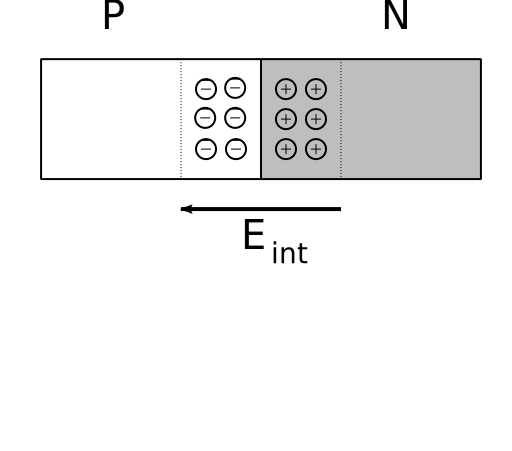
\includegraphics[width=0.80\textwidth]{./pics/pnjunction_nobias}
    \end{figure}
  \end{column}
  \begin{column}<2->{.3\textwidth}
    Reverse bias
    \begin{figure}
      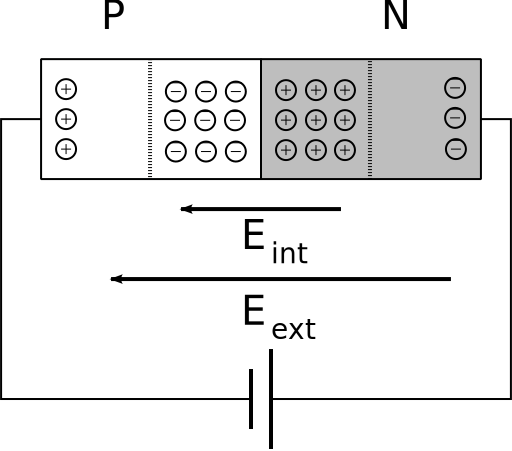
\includegraphics[width=0.80\textwidth]{./pics/pnjunction_reverse_bias}
    \end{figure}
  \end{column}
  \begin{column}<3->{.3\textwidth}
    Forward bias
    \begin{figure}
      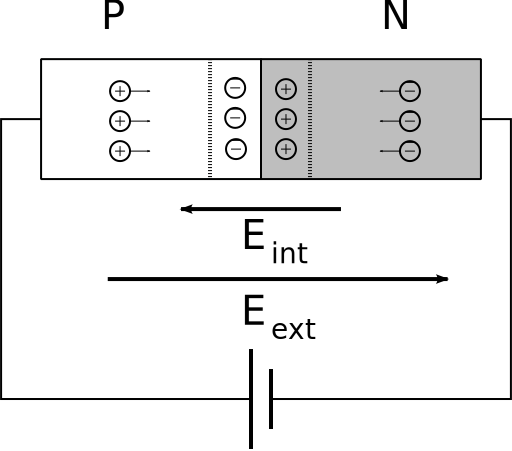
\includegraphics[width=0.80\textwidth]{./pics/pnjunction_forward_bias}
    \end{figure}
  \end{column}
 \end{columns}
\end{frame}

\begin{frame}
\frametitle{Diodes}
\vskip -.2in
\begin{figure}
  \includegraphics[width=0.30\textwidth]{./schematics/diode}
\end{figure}
\vskip -.2in
\begin{columns}[t]
  \begin{column}{.35\textwidth}
   \[
    I(V)=I_S\left( e^{{V}/(m V_{T})}-1 \right) 
   \]
   Typical parameters
   \begin{itemize}
    \item saturation current $I_S=1$~nA
    \item thermal voltage $V_T=\frac{kT}{q}=25.85$~mV at 300~K
    \item emission coefficient $m=1..2$
   \end{itemize}
  \end{column}
  \begin{column}{.65\textwidth}
    \begin{figure}
      \includegraphics<1>[angle=0,width=1.00\textwidth]{./plots/realistic_diode}
      \includegraphics<2>[angle=0,width=1.00\textwidth]{./plots/diode_combined}
    \end{figure}
  \end{column}
\end{columns}
\end{frame}

\begin{frame}
\frametitle{Simple NPN-transistor rules}
\begin{columns}[t]
 \begin{column}{.75\textwidth}
  To support shown currents direction
  \begin{itemize}
   \item \alert{$V_{ce} > 0$}
   \item \alert{$V_{be} > 0$}
    \begin{itemize}
     \item since, it is forward biased diode $V_{be} \approx 0.6$~V
    \end{itemize}
   \item \alert{$V_{cb} > 0$}
    \begin{itemize}
     \item since, it is reversed biased diode, no current goes from
      collector to base, all collector current is directed to emitter 
     \item if \textcolor{blue}{$V_{cb} < 0$} transistor goes to
      \textcolor{blue}{saturation} and cannot be
      described by the following simple rule.
    \end{itemize}
  \end{itemize}
  If above holds true then
  \begin{itemize}
   \item \alert{$I_{ce}=\beta I_{be}$} thus a BJT is a current
    amplifier
   \item {\it the static forward current transfer ratio}\\
    $\beta$ (or sometimes $h_{fe}$)   $\approx 100 \ldots 200$ 
   \item $I_e = I_{be} + I_{ce} = (\beta+1) I_{be} \approx \beta I_{be}$
  \end{itemize}
 \end{column}
 \begin{column}{.25\textwidth}
  \begin{figure}
   \includegraphics[width=0.80\textwidth]{./schematics/npn_transistor_with_currents.pdf}
  \end{figure}
  \begin{figure}
   \includegraphics[width=0.40\textwidth]{./schematics/npn_diodes.pdf}
  \end{figure}
 \end{column}
\end{columns}
\end{frame}
 
\begin{frame}{Transistors: Example}
 Consider the diagram shown below with a sinusoidal input signal $v_{in}$ with an amplitude of 0.01\,V and $V_{CC} = 15 V$.
 \begin{center}
  \begin{circuitikz}[scale=0.9,transform shape]
   \draw (4,4) node[npn](npn1){} node{$T_1$};
   \draw (8,5) node[npn](npn2){} node{$T_2$};
   \draw (0,4) node[anchor=east]{$v_{in}$} to[C,l=$C_1$,o-*] (2,4) to[short] (npn1.B);
   \draw (npn1.E) -| (4,3);
   \draw (4,3) to[short,*-] (3,3) to[R,l=$R_E$,-*] (3,1);
   \draw (4,3) to[short,*-] (4.5,3) to[C,l=$C_E$,-*] (4.5,1);
   \draw (2,1) to[R,l=$R_2$] (2,4) to[R,l=$R_1$] (2,7) to[short] (4,7) to[short] (6,7) -| (npn2.C);
   \draw (4,7.5) node[anchor=south]{$V_{CC}$} to[short,o-*] (4,7) to[R,l=$R_C$,*-] (npn1.C) |- (4,5) to[C,l=$C_2$,*-*] (6,5) to[short] (npn2.B);
   \draw (6,7) to[R,l=$R_3$,*-*] (6,5) to[R,l=$R_4$,*-*] (6,1);
   \draw (npn2.E) |- (8,4) to[C,l=$C_3$,*-o] (10,4) node[anchor=west]{$v_{out}$};
   \draw (2,1) to[short] (4.5,1) node[ground]{} to[short] (6,1) to[short] (8,1) to[R,l=$R_e$,-*] (8,4);
  \end{circuitikz}
 \end{center}
\end{frame}
 
\begin{frame}{Transistors: Example}
 \begin{itemize}
  \item What does this circuit do?  Identify any subcircuits that perform separate functions.
  \item Explain the purpose of the three capacitors $C_1$, $C_2$ and $C_3$.
  \item Explain the purpose of the capacitor $C_E$.
  \item Which values would you pick for $R_1$, $R_2$, $R_C$, $R_E$, $R_3$ and $R_4$ to achieve an amplification factor of at least 100?
 \end{itemize}
\end{frame}

\begin{frame}{Op Amps}
Consider the two modified non-inverting amplifier diagrams shown below:
 \begin{columns}
  \begin{column}{0.5\textwidth}
   \begin{center}
    \begin{circuitikz}[scale=0.6,transform shape]
     \draw (3,0.5) node[op amp](opamp){} node[left=0.1] {$A$};
     \draw (0,1) node[ground]{} to[R,l=$R_1$,-*] (opamp.-) |- (2.25,2) to[R,l=$R_2$] (3.75,2) -| (opamp.out);
     \draw (1.5,0) node[anchor=east]{$v_{in}$} to[short,o-] (opamp.+);
     \draw (opamp.out) to[short,*-] (4.5,0.5) to[R,l=$R_3$] (6.5,0.5) node[anchor=west]{$v_{out}$};
    \end{circuitikz}
   \end{center}
  \end{column}
  \begin{column}{0.5\textwidth}
   \begin{center}
    \begin{circuitikz}[scale=0.6,transform shape]
     \draw (3,0.5) node[op amp](opamp){} node[left=0.1] {$A$};
     \draw (0,1) node[ground]{} to[R,l=$R_1$,-*] (opamp.-) |- (2.25,2) to[R,l=$R_2$] (3.75,2) -| (6.0,0.5);
     \draw (1.5,0) node[anchor=east]{$v_{in}$} to[short,o-] (opamp.+);
     \draw (opamp.out) to[R,l=$R_3$] (6.0,0.5) to[short,*-] (6.5,0.5) node[anchor=west]{$v_{out}$};
    \end{circuitikz}
   \end{center}
  \end{column}
 \end{columns}
 Assume that all op amps are ideal (with open loop gain $A = \infty$).
 \begin{itemize}
  \item Express $v_{out}$ as a function of $v_{in}$ and circuit components assuming no load is connected.
  \item Express $v_{out}$ as a function of $v_{in}$ and circuit components when a load $R_L$ is connected.
  \item What is the output impedance of these circuits?
 \end{itemize}
\end{frame}

\begin{frame}{Functional feedback}
 \begin{figure}
  \includegraphics[width=0.5\textwidth]{./pics/functional}
 \end{figure}
 \begin{block}{}
  \begin{eqnarray*}
   i(v_{diode}) & = & I_S (e^{v/V_T} - 1) \\
   v_{diode}(i) & = & \ln(1 + i/I_S)
  \end{eqnarray*}
 \end{block}
\end{frame}

\end{document}
